%\subsection{Appendix 1}\label{app:A1}

The following four figures complement the dynamic analysis of \autoref{sec:results}. \autoref{fig:continuumheat} shows the full results of the one-week-ahead ($h=1$) response of the government bond yield at each maturity to a one-standard-deviation restrictive ECB surprise, evaluated at each percentile of the US monetary policy stance. \autoref{fig:IRFswps} and \autoref{fig:IRFreal} report the dynamic responses of inflation swaps and real yields under the two reference stances of the Fed, whose one-week-ahead behavior across the full stance continuum is summarized in \autoref{fig:headline} in the main text.

\begin{figure}[!htpb]
\centering
\caption{Heatmap of one-week-ahead response of the full government bond yield curve to a restrictive ECB surprise, across all percentiles of the Fed's monetary policy stance.\label{fig:continuumheat}}
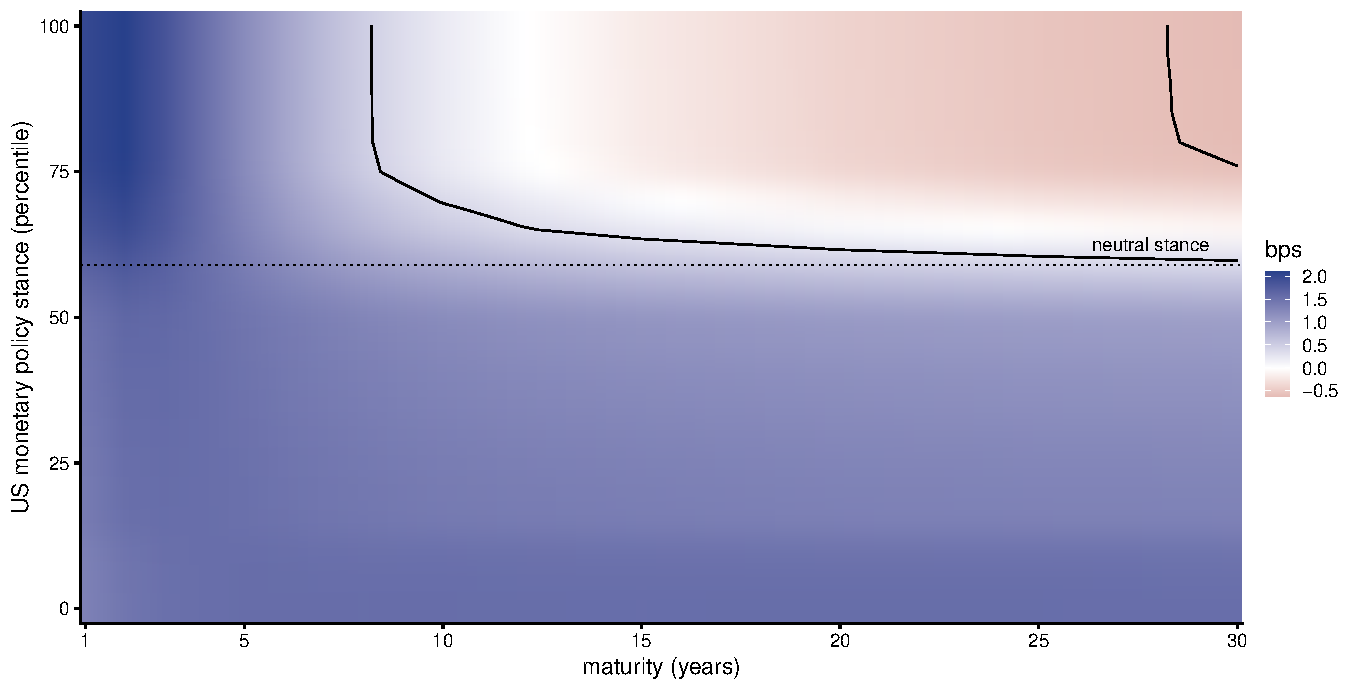
\includegraphics[width=\textwidth]{images_updated/rev/IRF_termstructure_continuum.pdf}
\caption*{\footnotesize \textit{Notes:} Posterior median of the one-week-ahead ($h=1$) response (in basis points, color scale) of the government bond yield at each maturity (horizontal axis, 1-30 years) to a one-standard-deviation restrictive ECB surprise, evaluated at each percentile of the US monetary policy stance $z^\ast_t$ (vertical axis; 0 = most accommodative, 100 = most restrictive week in the sample). The solid contour delimits the region in which the $68\%$ posterior credible set no longer excludes zero (upper right); the dotted horizontal line marks the percentile at which the stance crosses zero, i.e., the calibrated regime threshold. Responses at maturities between the 15 estimated grid points are linearly interpolated. Estimated on the nominal bond term structure over the full sample, 2005:W1-2025:W52.}
\end{figure}

The swap responses are an order of magnitude smaller than the yield responses and, beyond the impact week, the differences across Fed regimes are imprecisely estimated; the real-yield dynamics closely track the nominal ones. \autoref{fig:IRFcum} accumulates the weekly yield responses and displays the implied \textit{level} effects: since the model is specified in first differences of the term structure factors, a differenced response that returns to zero does not mean the effect on yields disappears, but that yields settle at a new level. Under an accommodative Fed, yields of three years and above settle about two basis points higher and the effect does not unwind over the 26-week horizon; under a restrictive Fed no lasting level effect remains, and the cumulated response of the one-year yield even drifts slightly negative, which is the level counterpart of the short-end reversal discussed in the main text.

\begin{figure}[!htpb]
\caption{Impulse responses of a restrictive EA monetary policy shock for selected \textit{inflation swaps}.\label{fig:IRFswps}}
\begin{minipage}{\textwidth}
\centering
a) Responses for two scenarios of US monetary policy
\end{minipage}
\begin{minipage}{\textwidth}
\centering
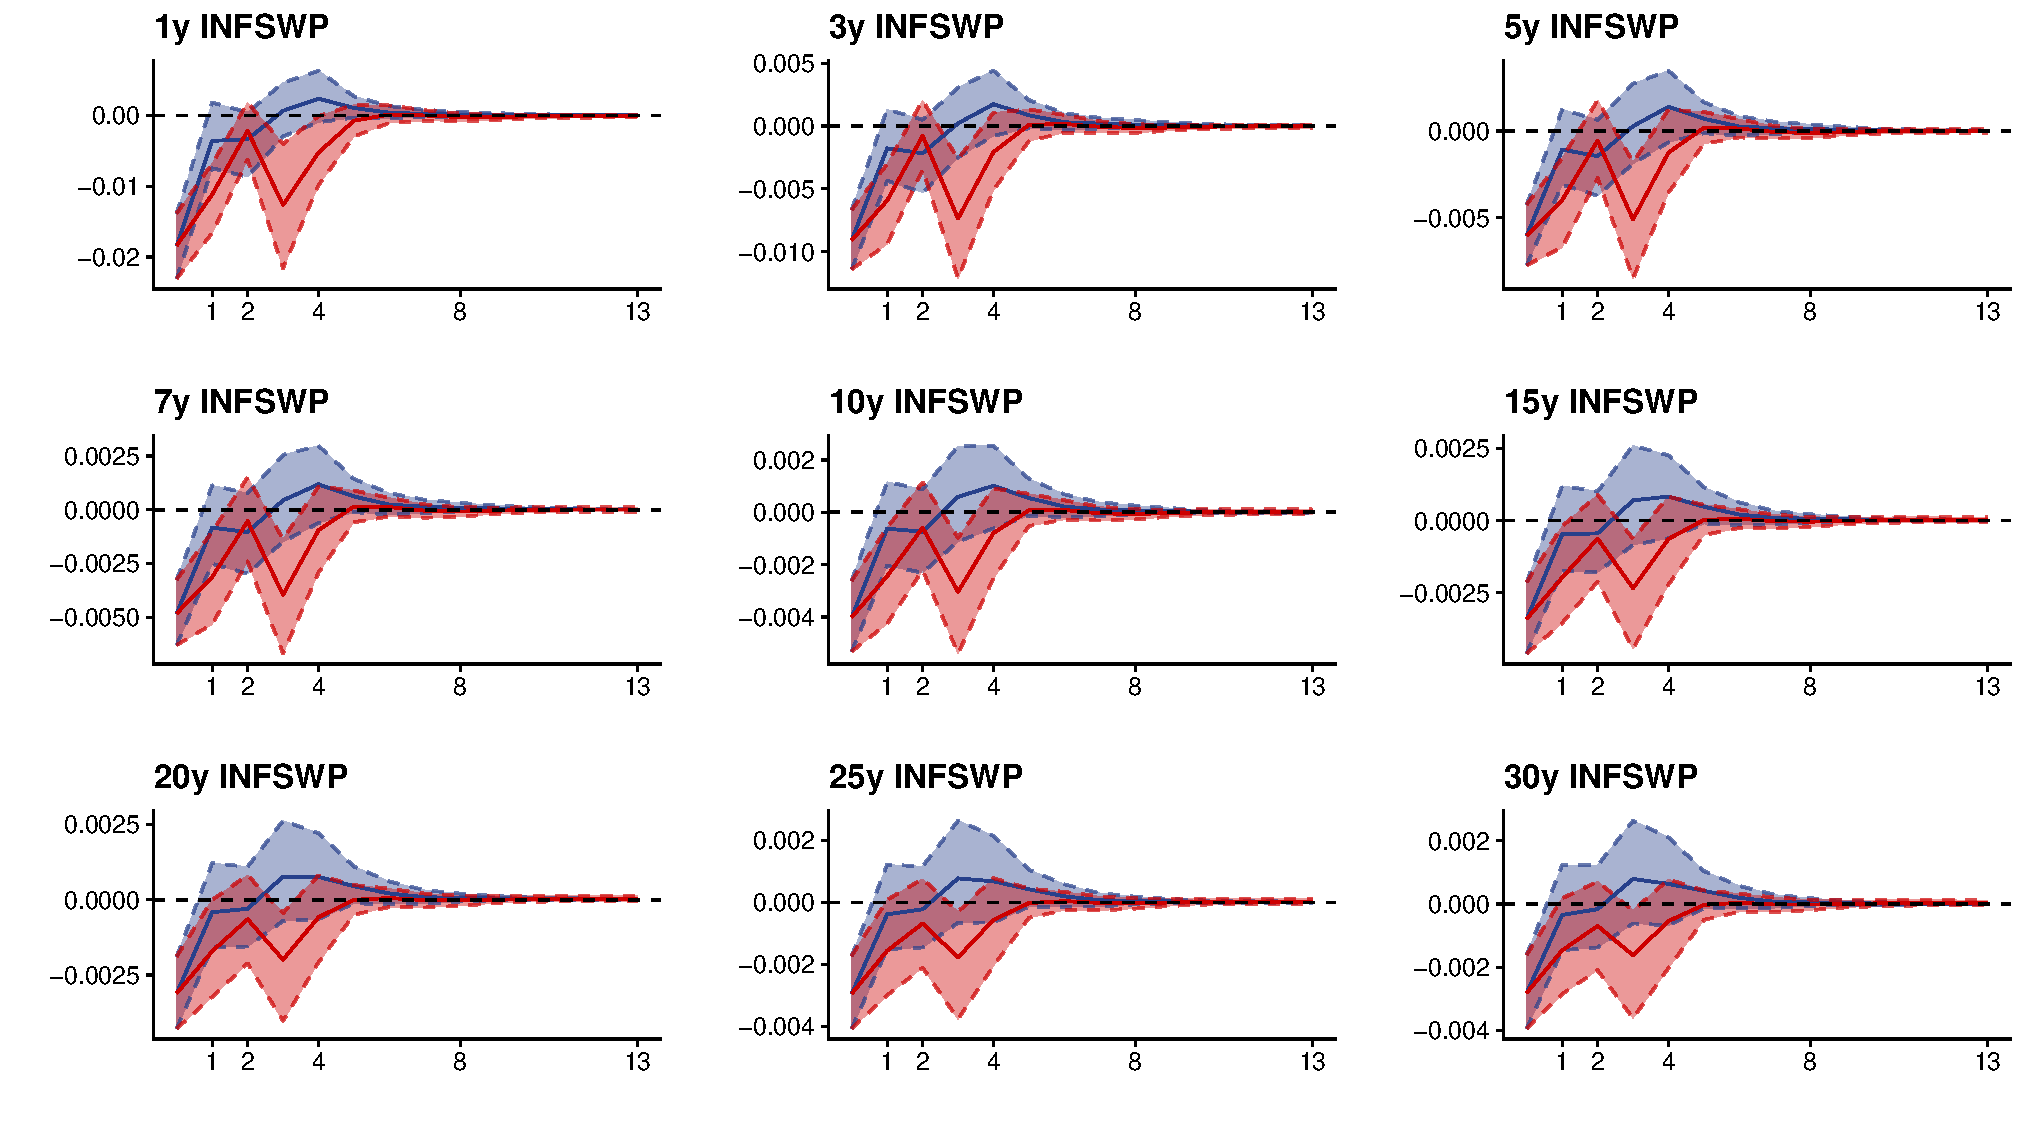
\includegraphics[width= 0.7\textwidth]{images_updated/DIFF_EA_Motto/IRF_INFSWP_LH_SLCT.pdf}
\end{minipage}
\begin{minipage}{\textwidth}
\centering
b) Difference in responses
\end{minipage}
\begin{minipage}{1\textwidth}
\centering
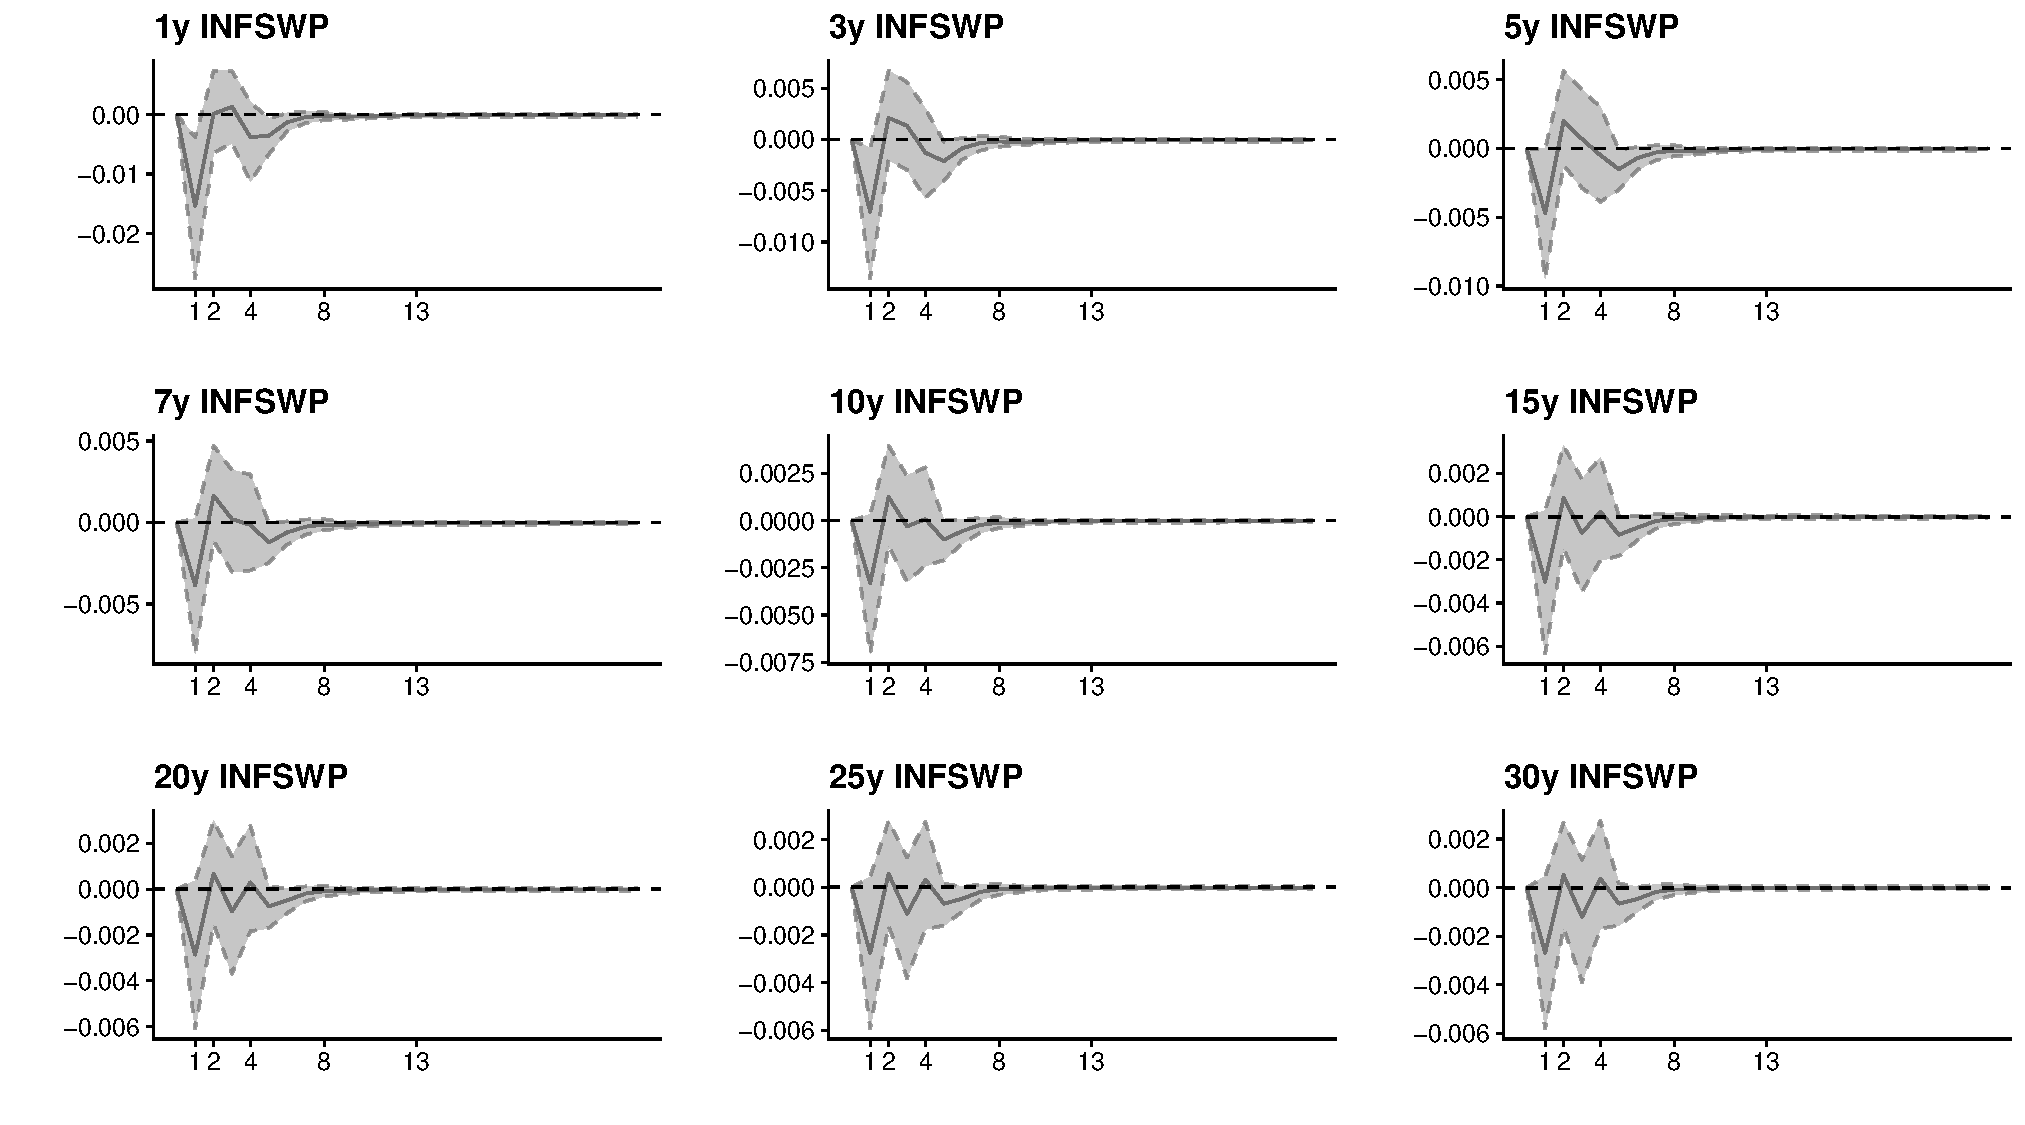
\includegraphics[width= 0.7\textwidth]{images_updated/DIFF_EA_Motto/IRF_INFSWP_D_SLCT.pdf}
\end{minipage}
\caption*{\footnotesize \textit{Notes:} Responses of inflation-linked swap rates to a contractionary EA monetary policy shock conditional on a restrictive US stance (95\% percentile of the threshold, red) and an expansionary US stance (5\% percentile, blue); panel (b) shows the difference (restrictive minus expansionary). The horizontal axis indicates weeks after the shock; shaded areas denote the 68\% posterior credible set.}
\end{figure}

\begin{figure}[!htpb]
\caption{Impulse responses of a restrictive EA monetary policy shock for selected\textit{ real rates}.}\label{fig:IRFreal}
\begin{minipage}{\textwidth}
\centering
a) Responses for two scenarios of US monetary policy
\end{minipage}
\begin{minipage}{\textwidth}
\centering
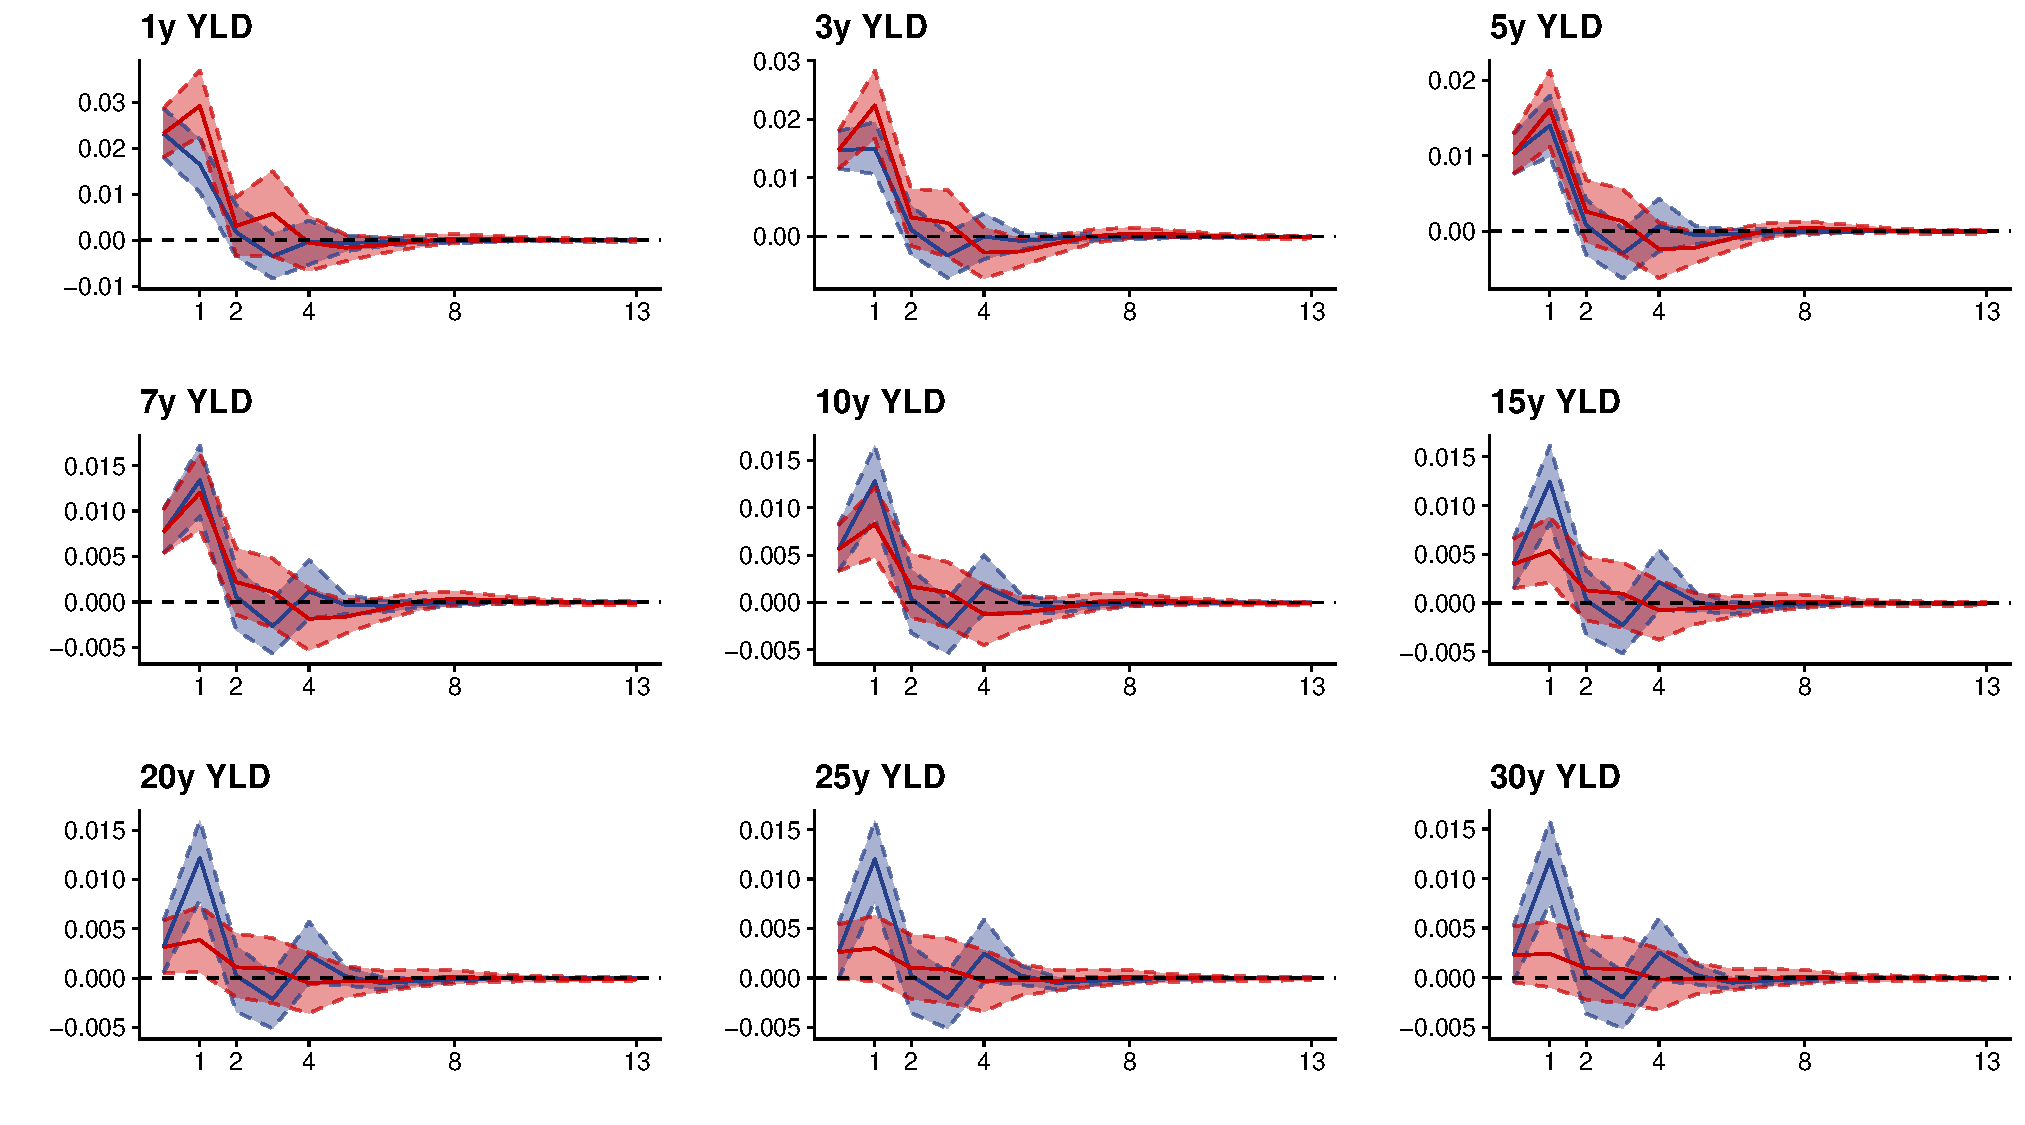
\includegraphics[width= 0.7\textwidth]{images_updated/DIFF_EA_real_Motto/IRF_YLDS_LH_SLCT.pdf}
\end{minipage}
\begin{minipage}{\textwidth}
\centering
b) Difference in responses
\end{minipage}
\begin{minipage}{1\textwidth}
\centering
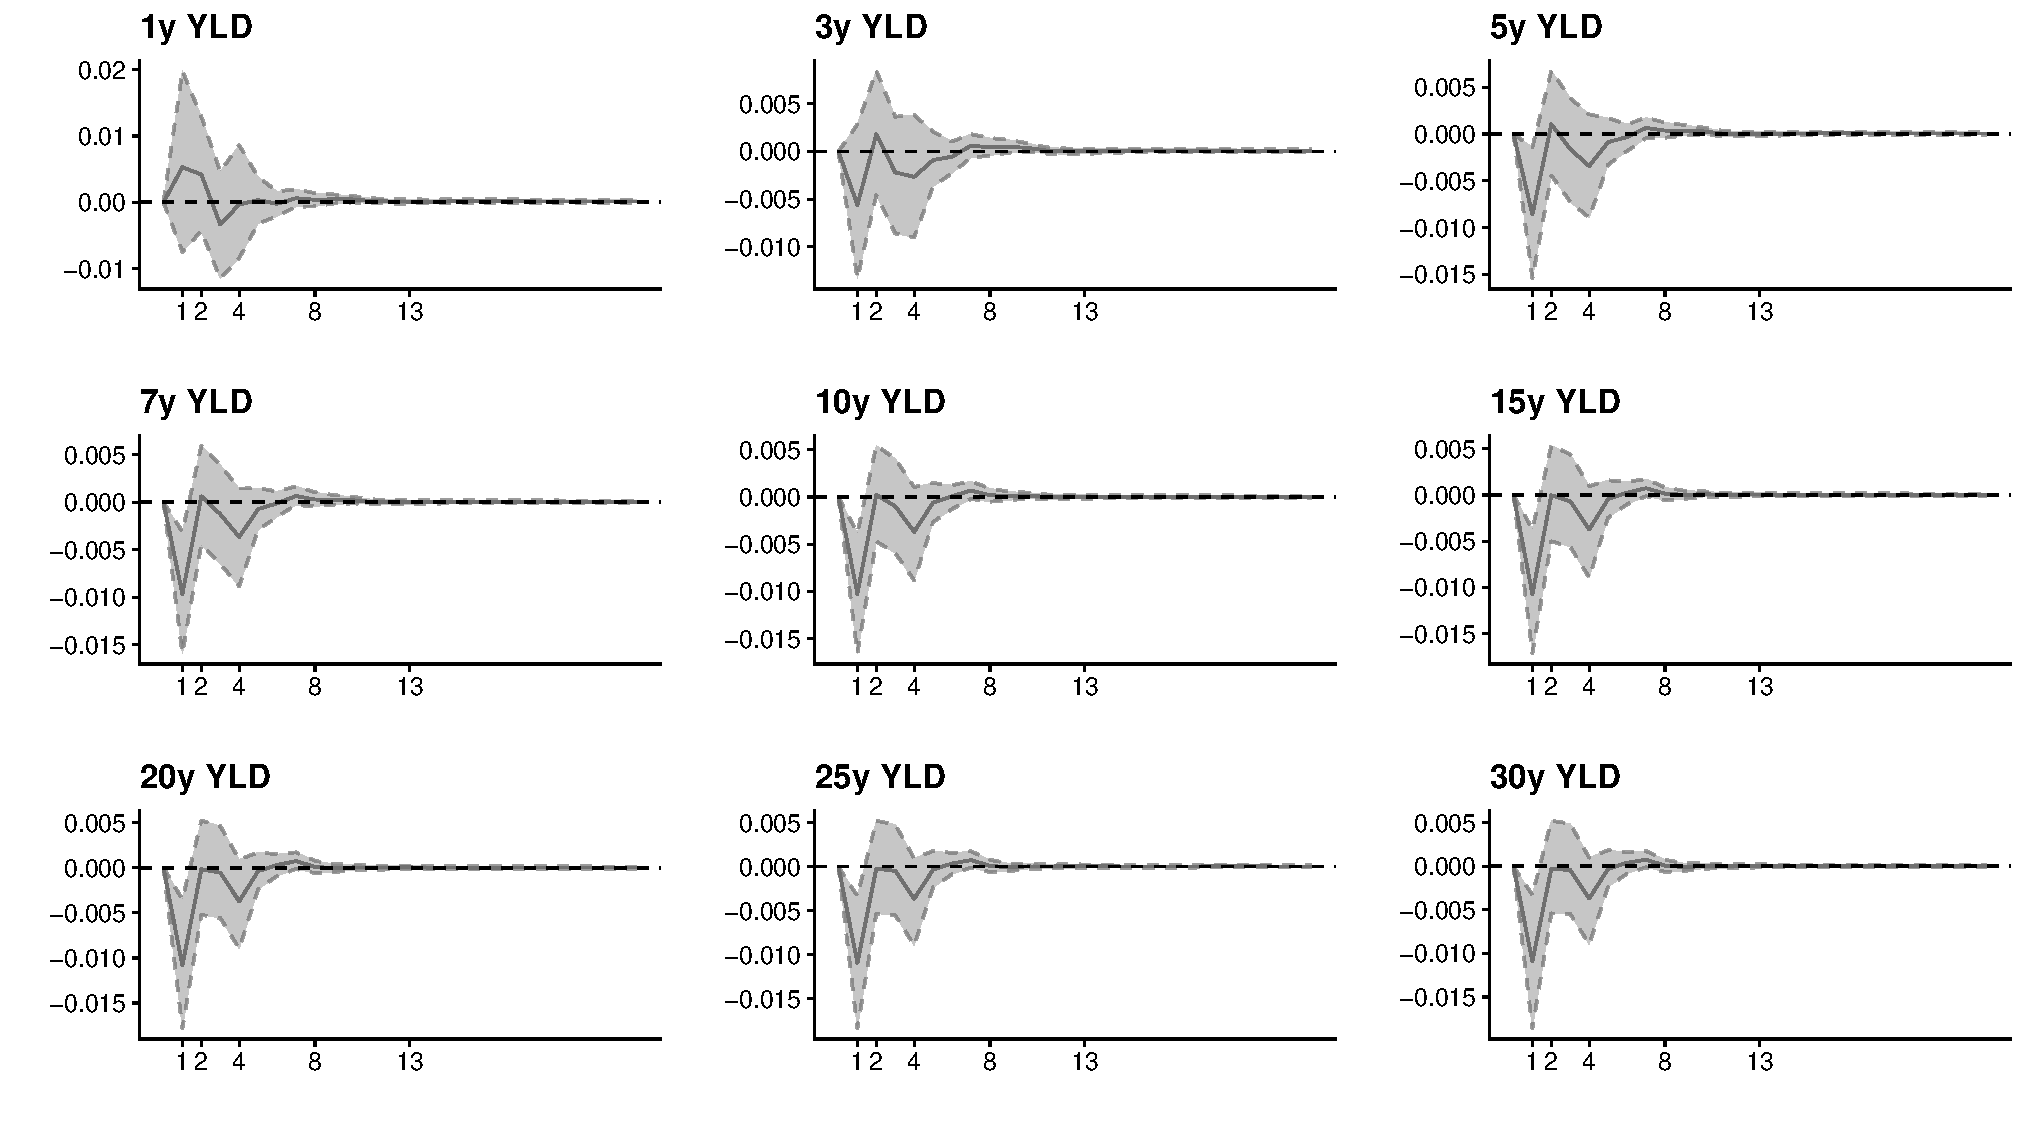
\includegraphics[width= 0.7\textwidth]{images_updated/DIFF_EA_real_Motto/IRF_YLDS_D_SLCT.pdf}
\end{minipage}
\caption*{\footnotesize \textit{Notes:} Responses of real yields (computed draw-wise as the nominal yield response minus the corresponding inflation swap response) to a contractionary EA monetary policy shock, conditional on a restrictive US stance (95\% percentile, red) and an expansionary US stance (5\% percentile, blue); panel (b) shows the difference. Shaded areas denote the 68\% posterior credible set.}
\end{figure}

\begin{figure}[!htpb]
\caption{Cumulated (level) responses of government bond yields to a restrictive EA monetary policy shock.\label{fig:IRFcum}}
\begin{minipage}{\textwidth}
\centering
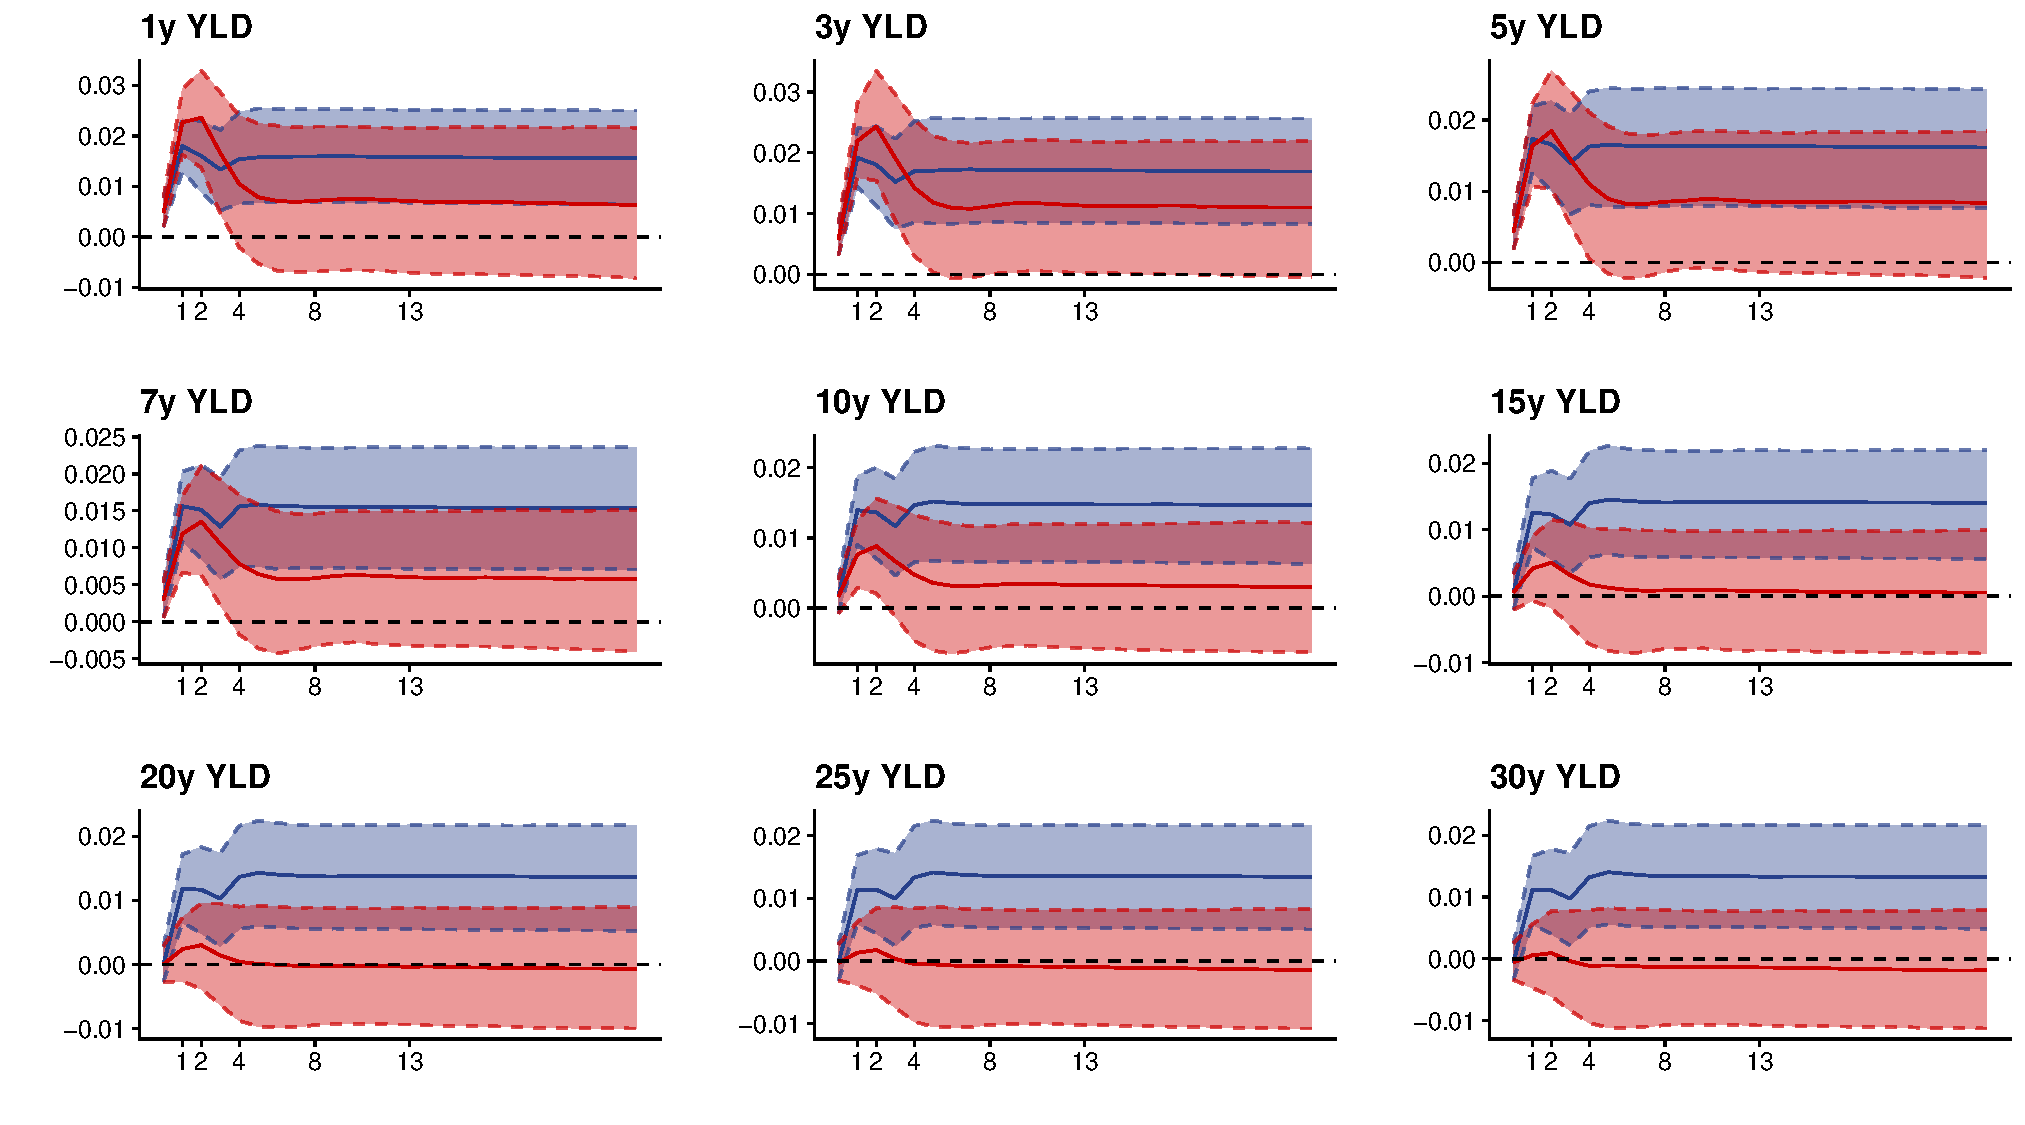
\includegraphics[width=0.85\textwidth]{images_updated/rev/IRF_YLDS_CUM_LH_SLCT.pdf}
\end{minipage}
\caption*{\footnotesize \textit{Notes:} Cumulated impulse responses (implied level effects, in percentage points) under a restrictive (95\% percentile, red) and an expansionary (5\% percentile, blue) US monetary policy stance, over the 26-week horizon. Shaded areas denote the 68\% posterior credible set.}
\end{figure}

% \begin{figure}[!htbp]
% \caption{Peak responses of a restrictive EA monetary policy shock for a set of US monetary policy scenarios.\label{fig:IRFpeaks}}
% \begin{minipage}{\textwidth}
% \centering
% a) Full yield curve
% \end{minipage}
% \begin{minipage}{\textwidth}
% \centering
% 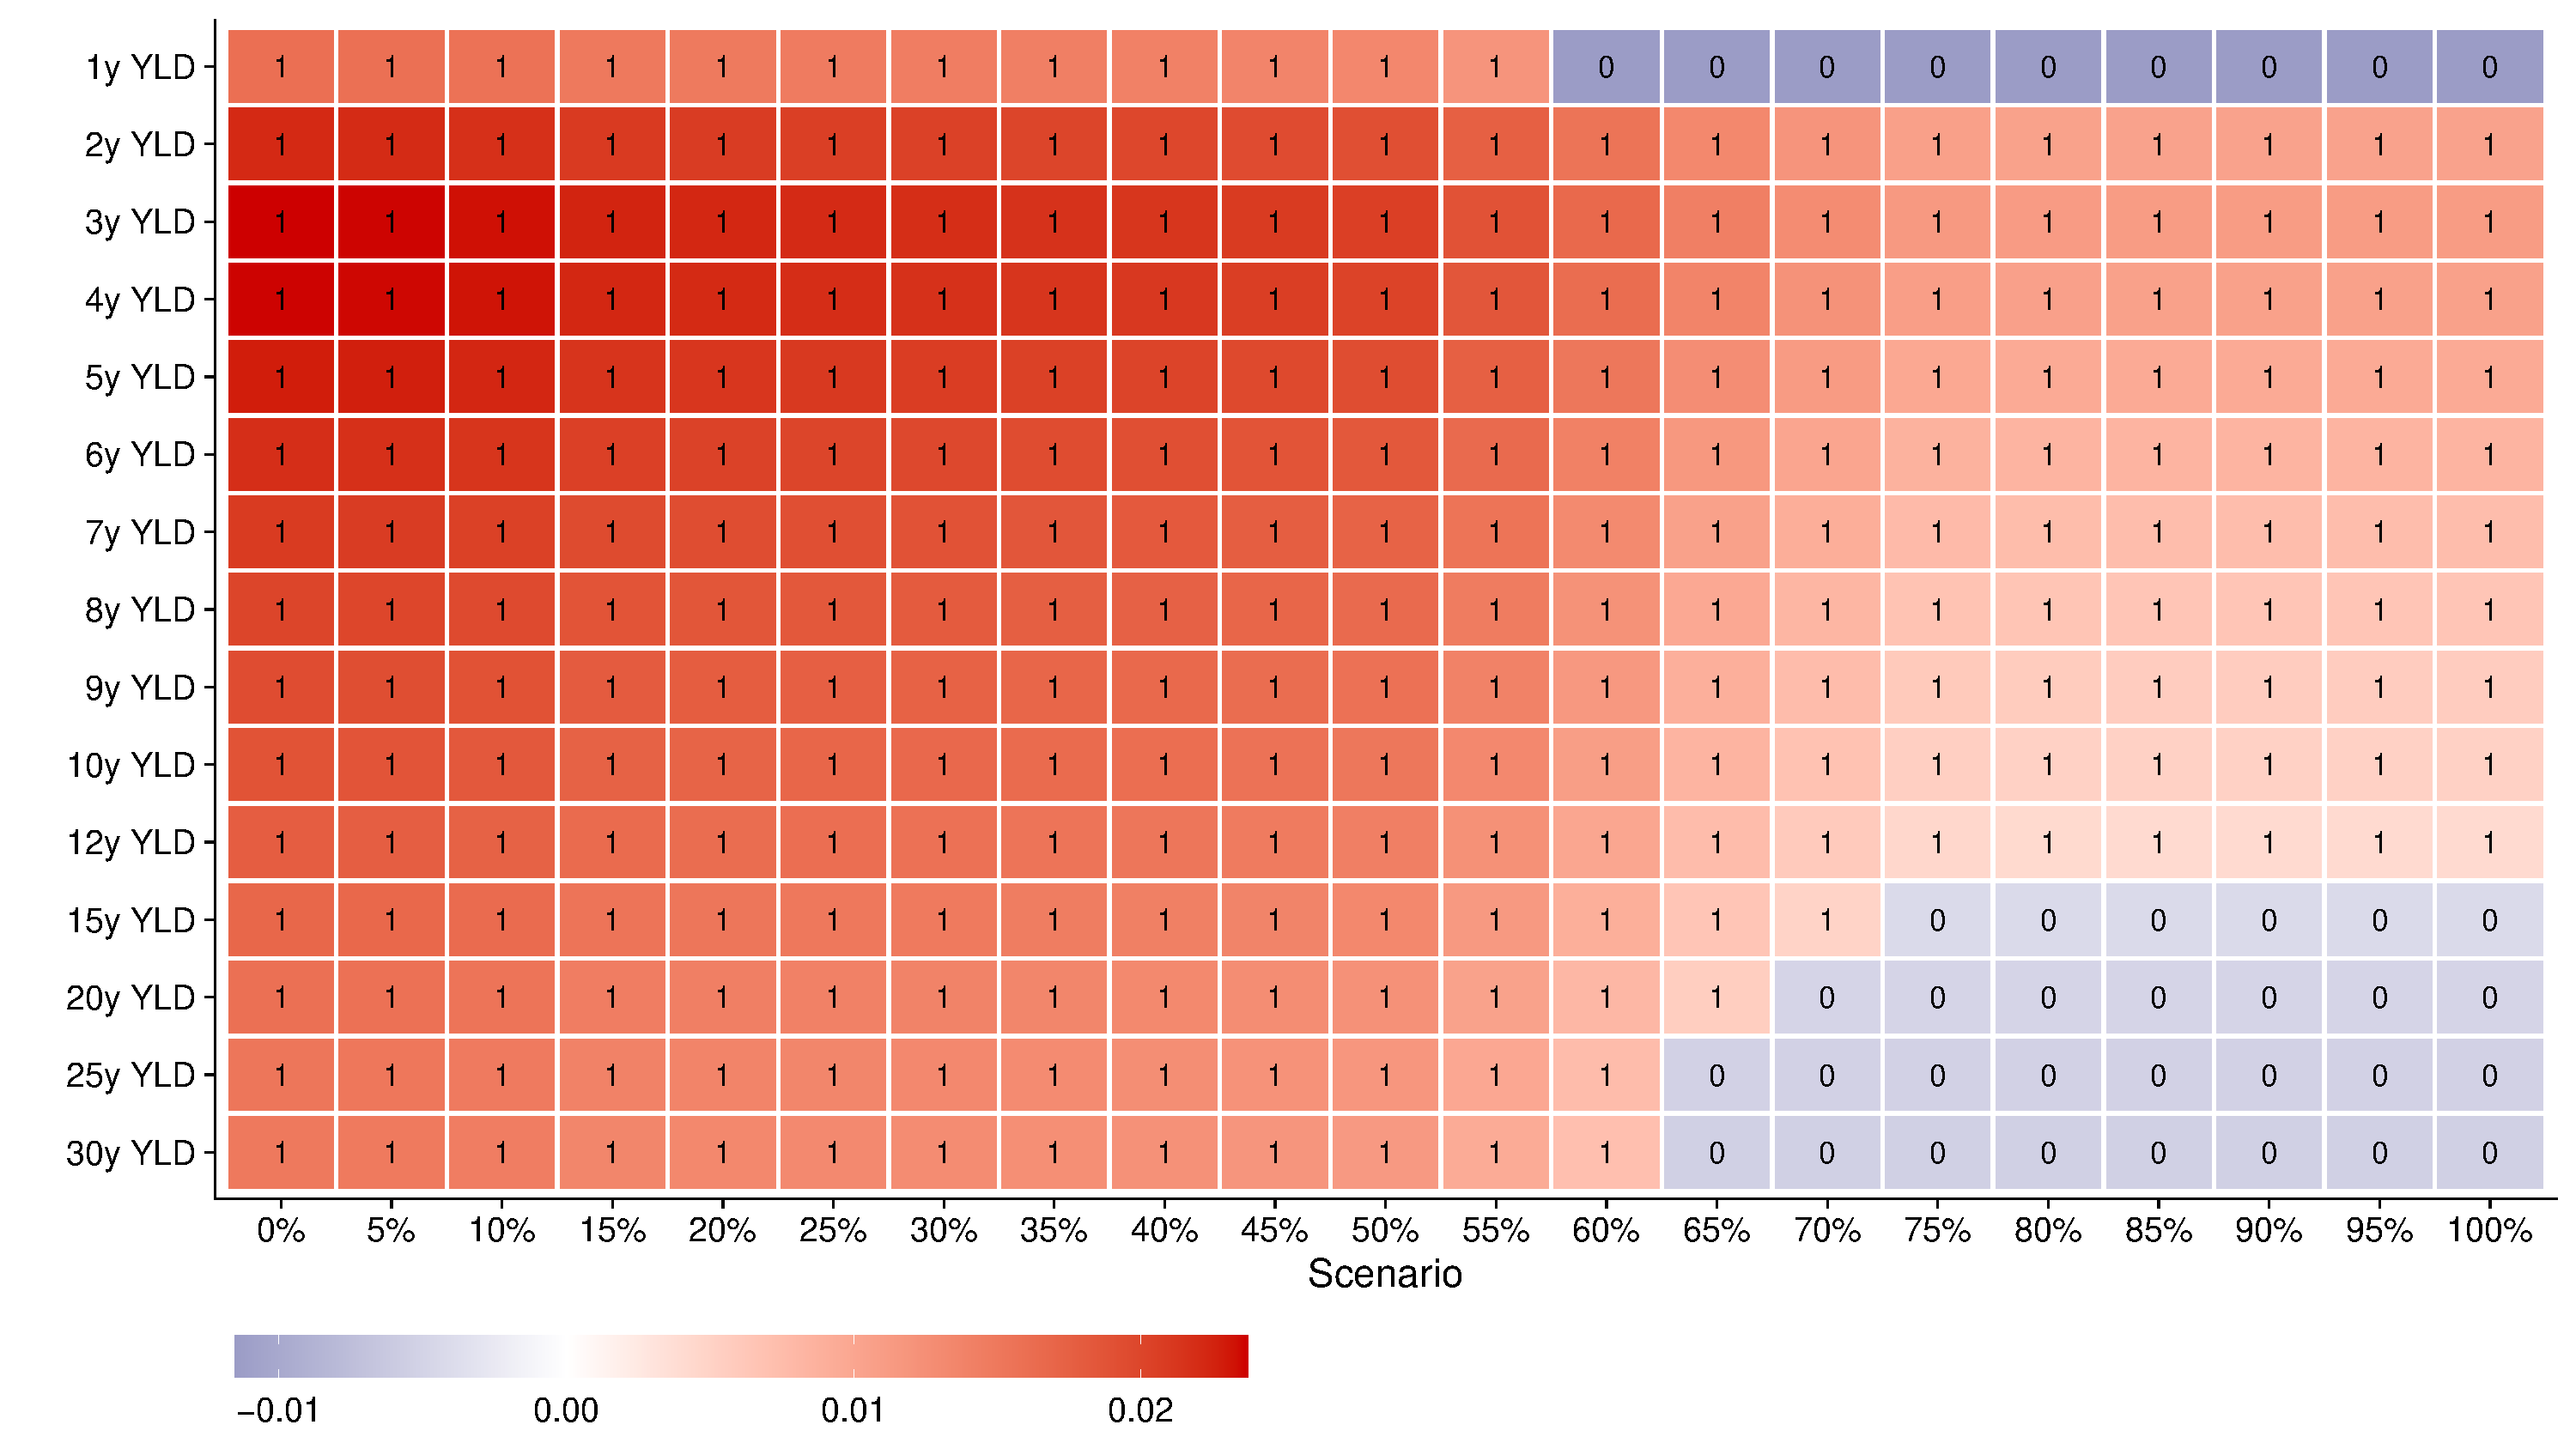
\includegraphics[width= 0.65\textwidth]{images_updated/DIFF_EA_Motto/IRF_YLDS_PEAK.pdf}
% \end{minipage}
% \begin{minipage}{\textwidth}
% \centering
% b) Inflation swaps
% \end{minipage}
% \begin{minipage}{1\textwidth}
% \centering
% 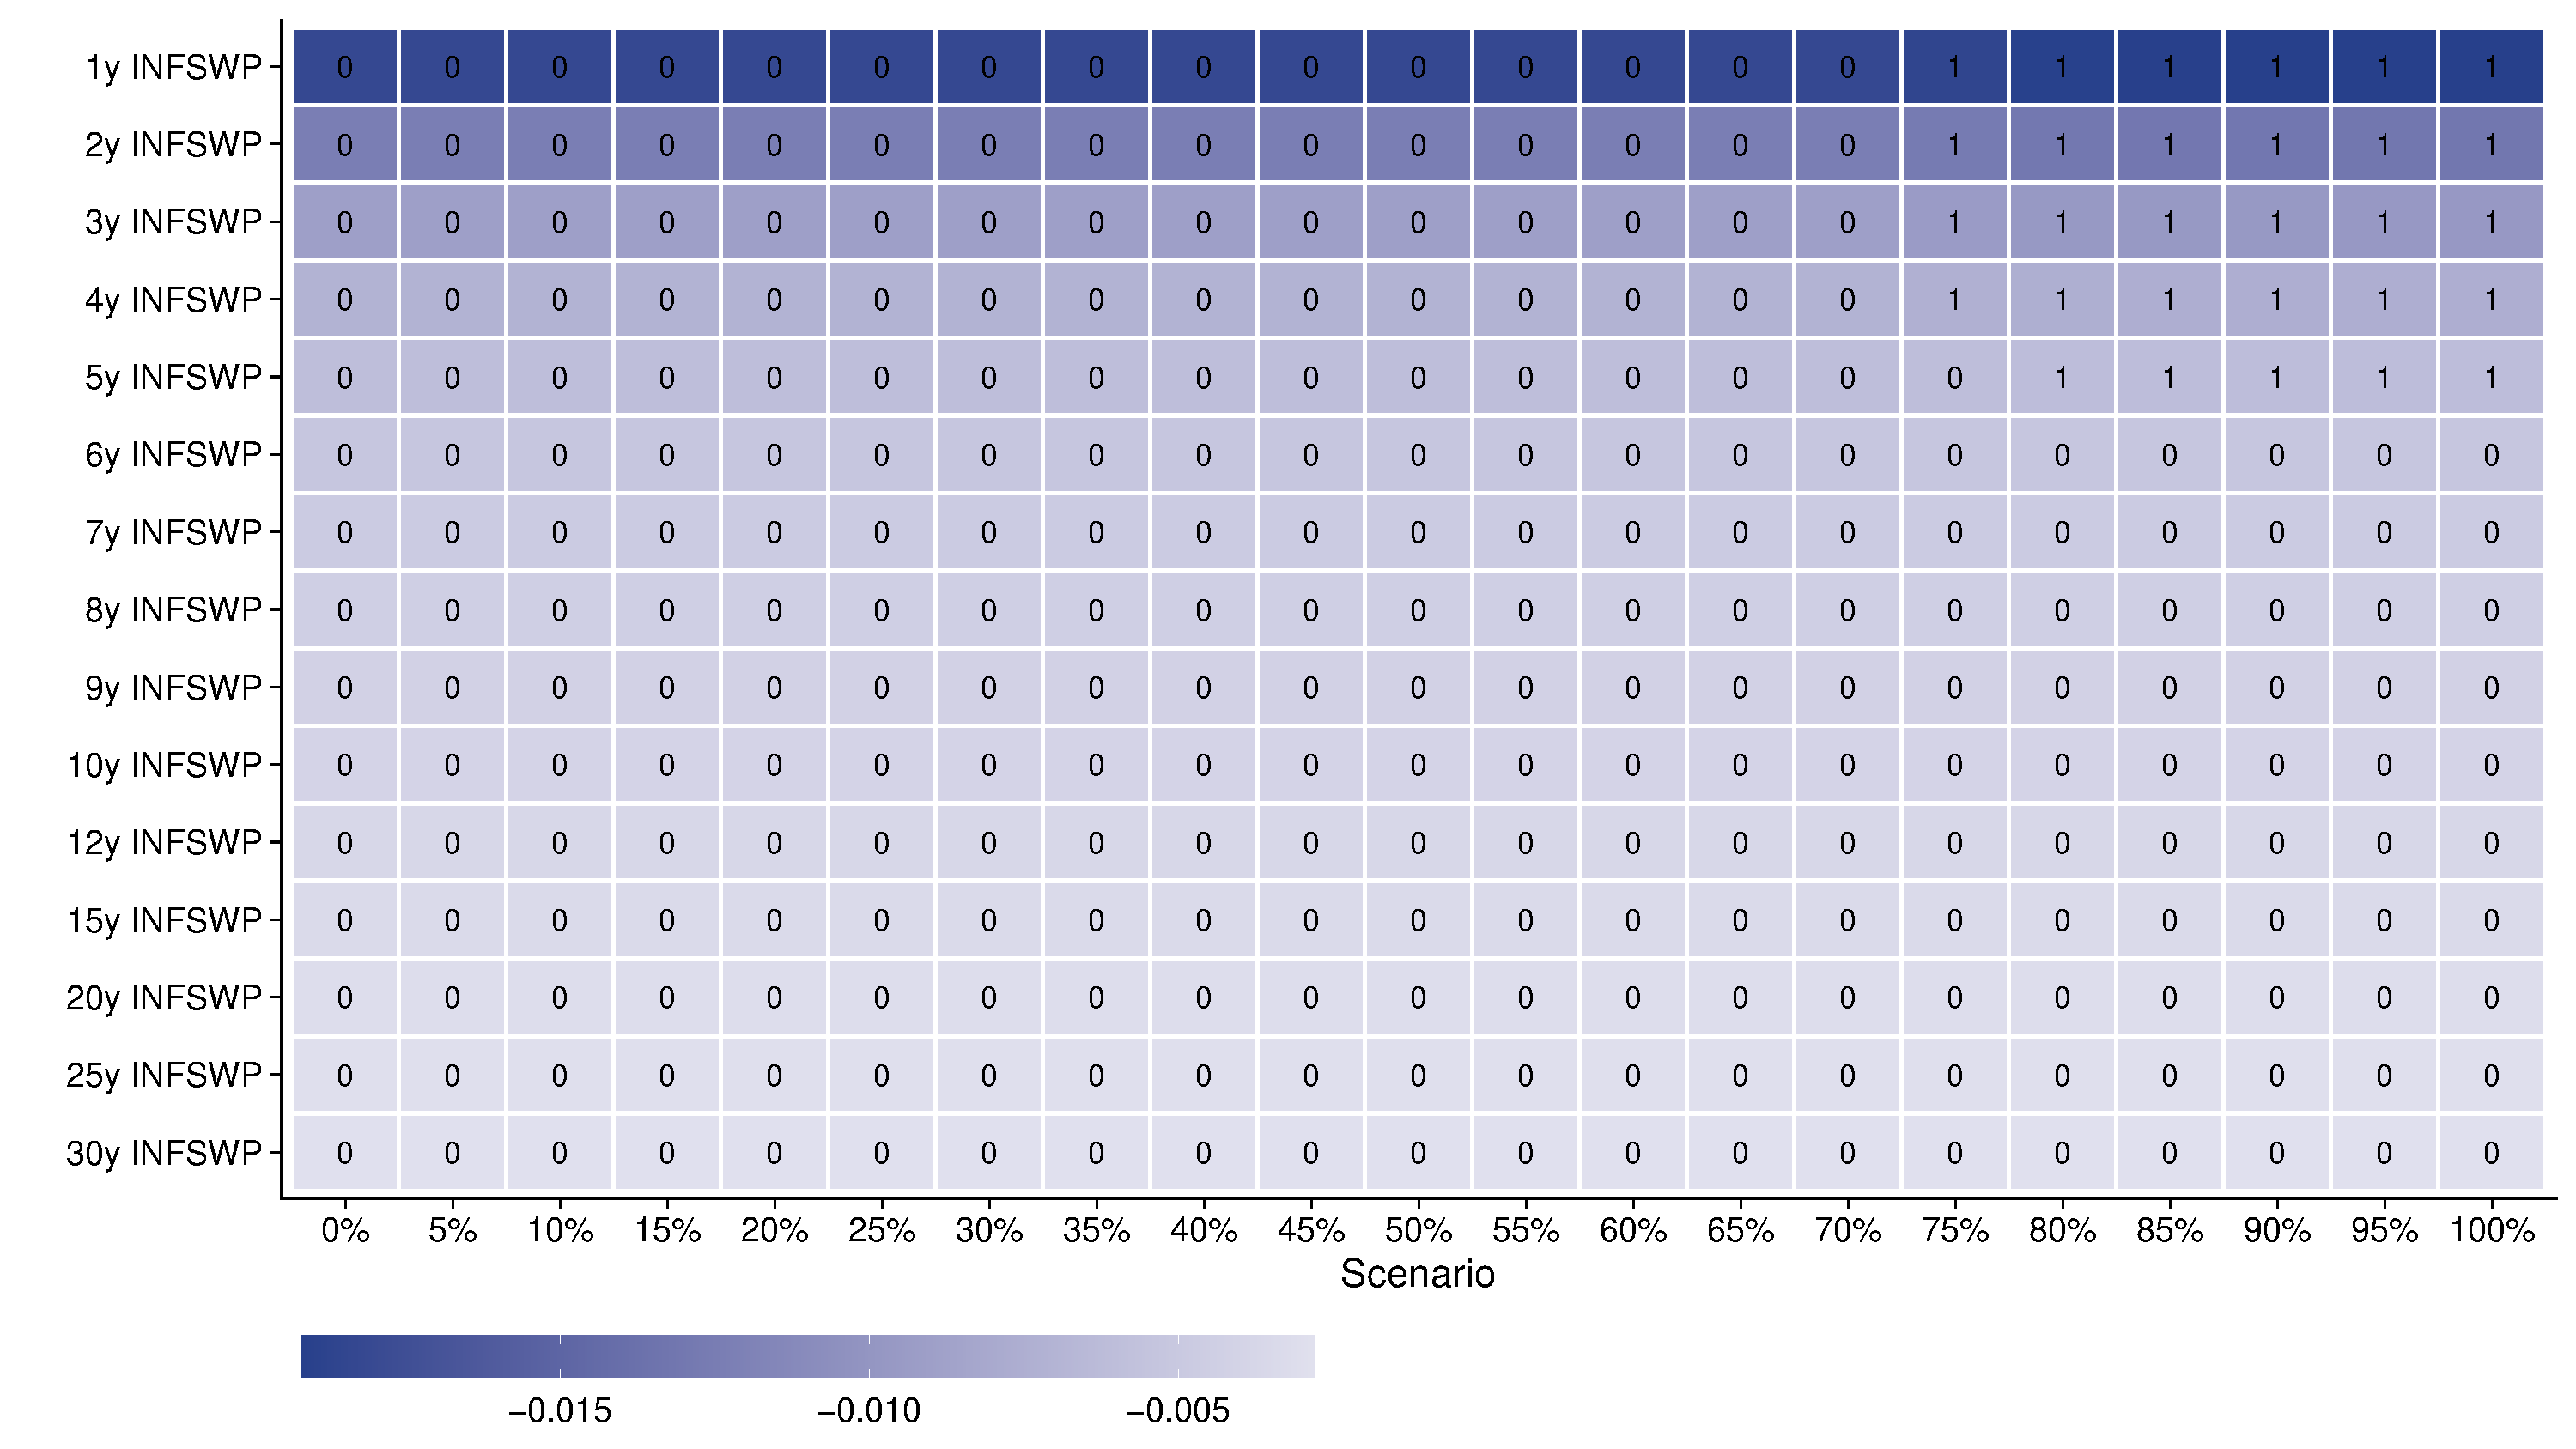
\includegraphics[width= 0.65\textwidth]{images_updated/DIFF_EA_Motto/IRF_INFSWP_PEAK.pdf}
% \end{minipage}
% \begin{minipage}{\textwidth}
% \centering
% c) Real rates (difference between government bond yields and inflation swaps)
% \end{minipage}
% \begin{minipage}{1\textwidth}
% \centering
% 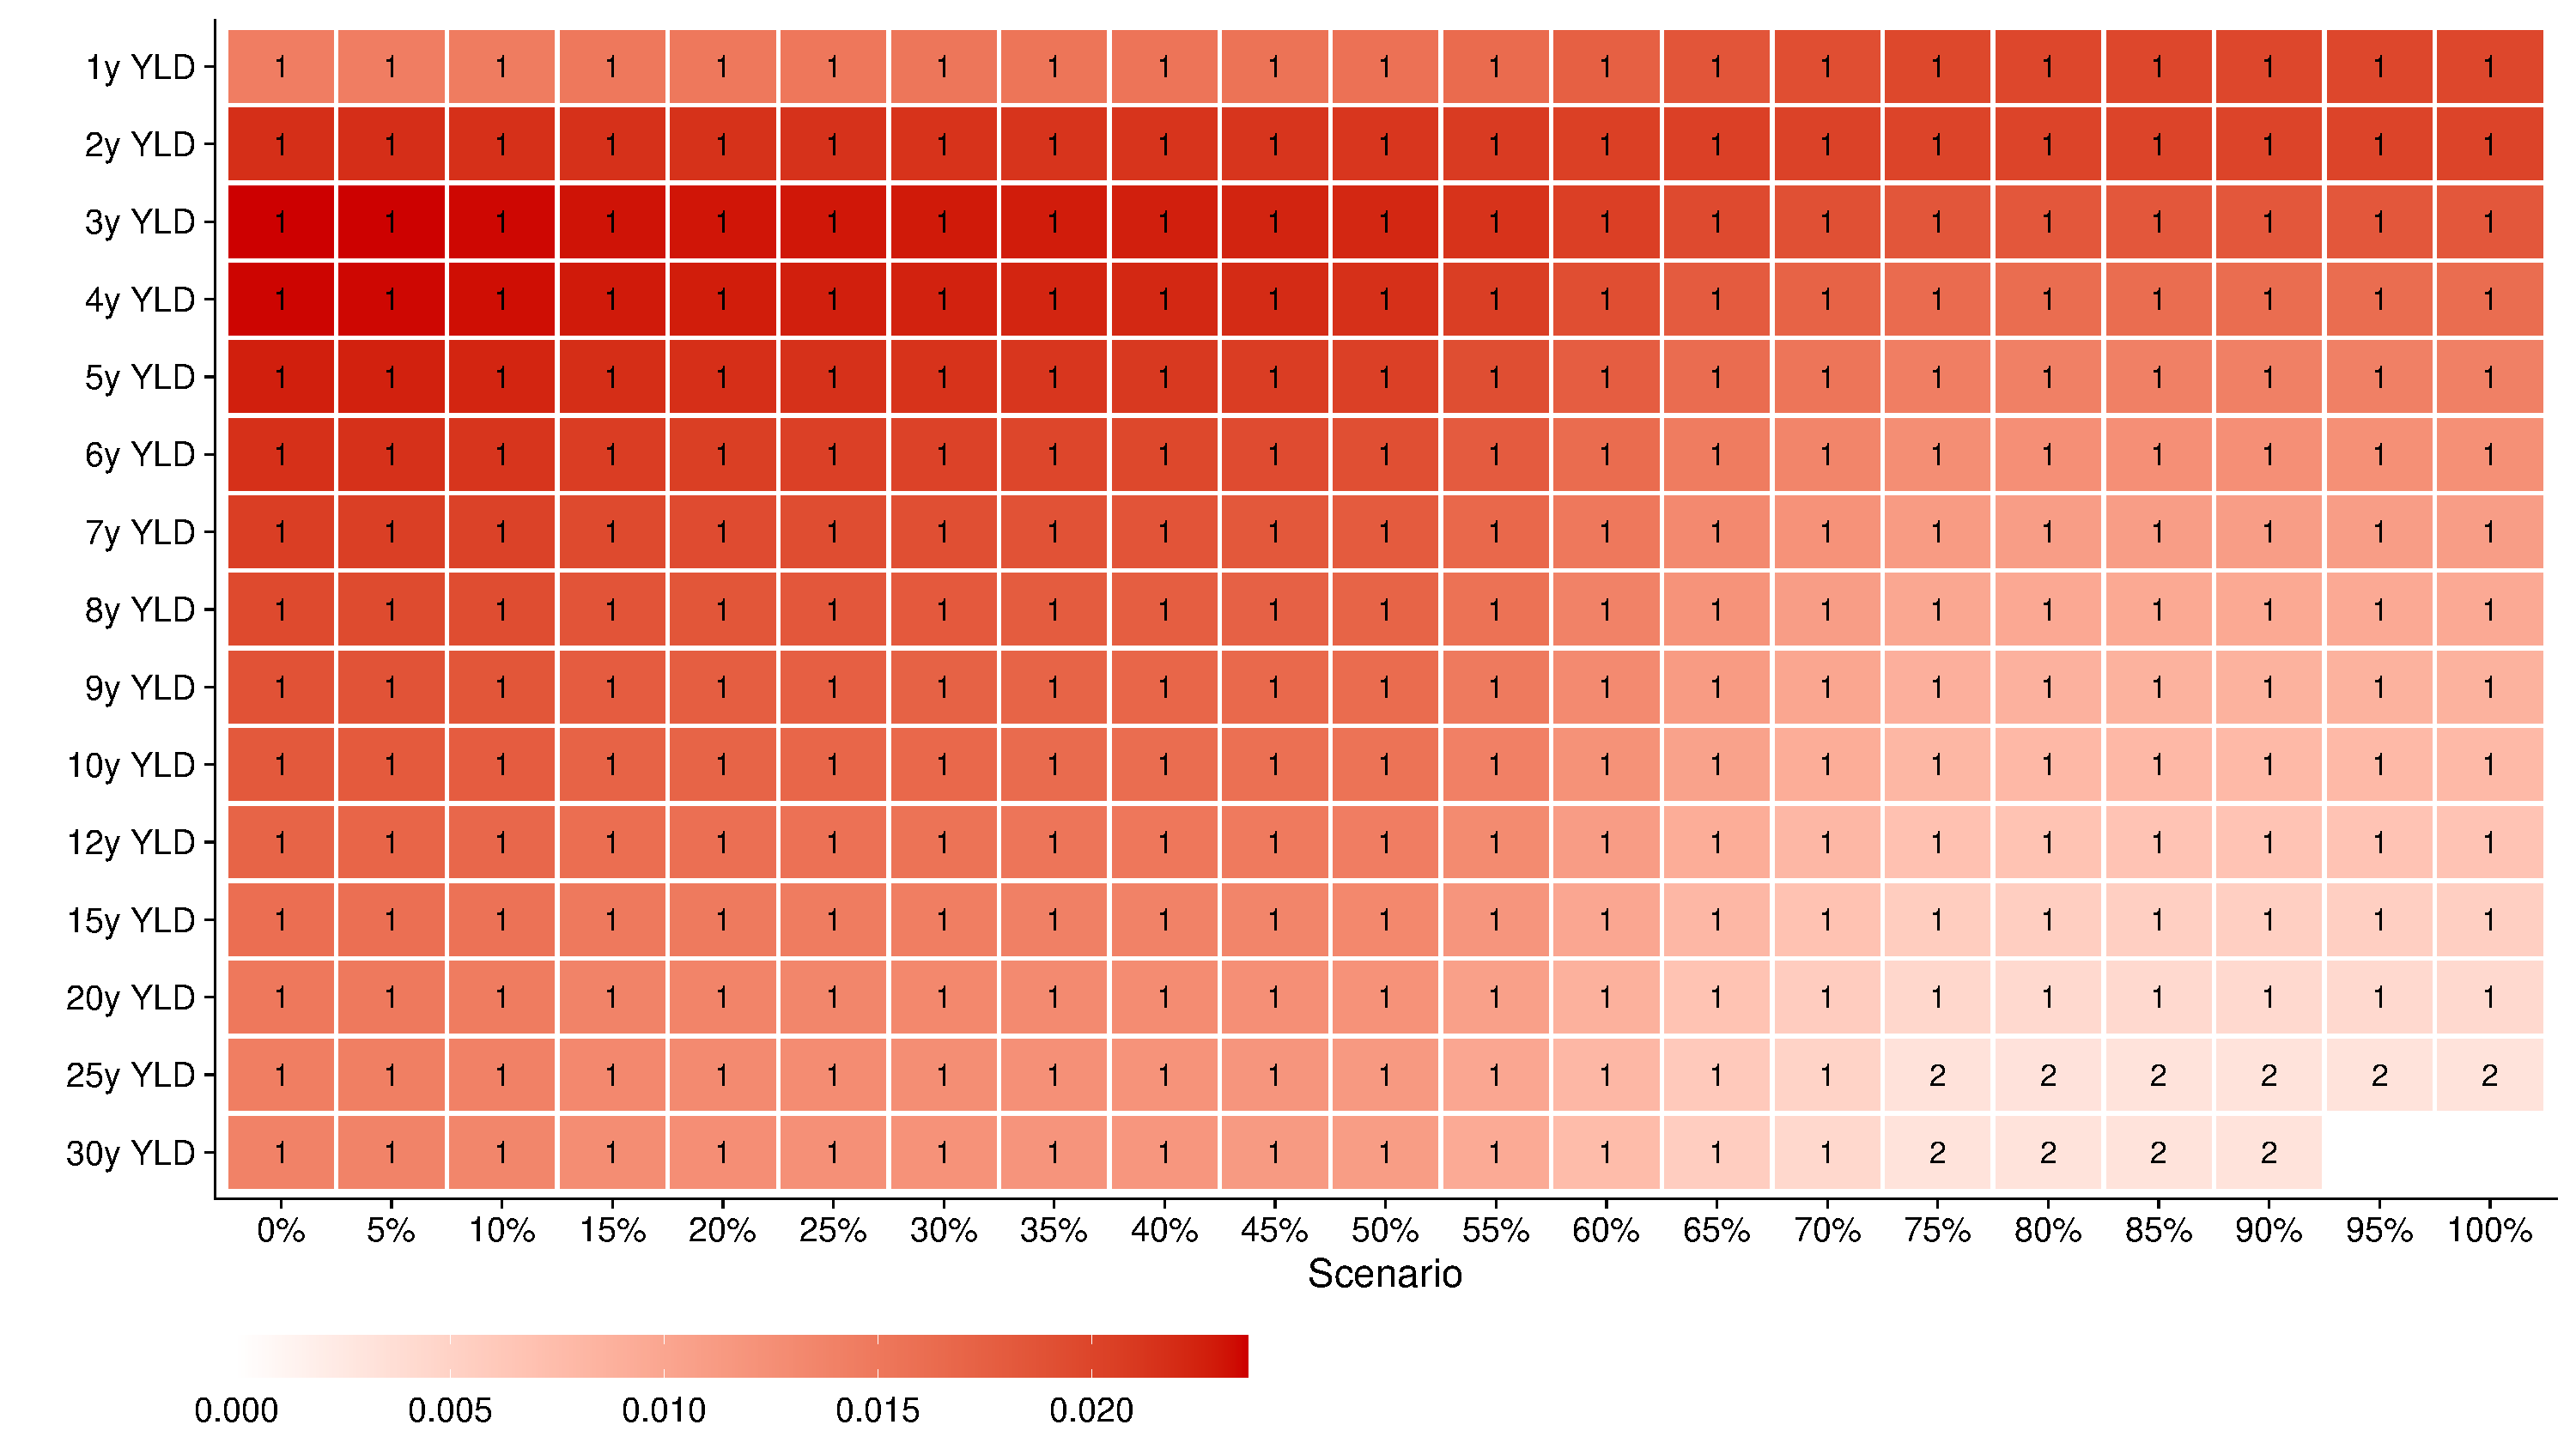
\includegraphics[width= 0.65\textwidth]{images_updated/DIFF_EA_real_Motto/IRF_YLDS_PEAK.pdf}
% \end{minipage}
% \begin{minipage}{\textwidth}
% \centering
% d) Other macrofincancial quantities
% \end{minipage}
% \begin{minipage}{1\textwidth}
% \centering
% 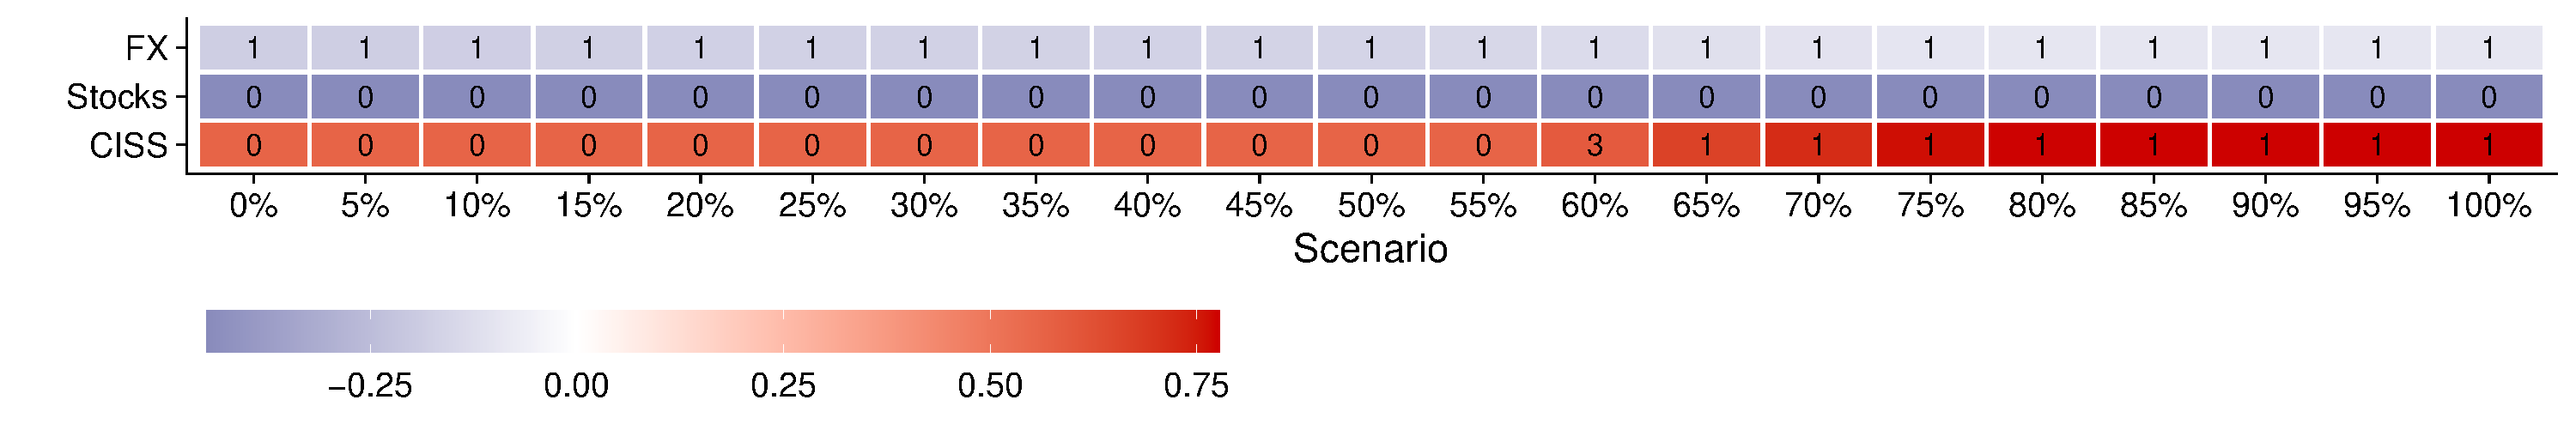
\includegraphics[width= 0.65\textwidth]{images_updated/DIFF_EA_Motto/IRF_OTHERS_PEAK.pdf}
% \end{minipage}
% \caption*{\footnotesize \textit{Notes:} While red (blue) shaded cells indicate significant negative (positive) peak responses, the cell number refers to the week after the shock at which the a significant response peaks. Significance is defined with respect to the $68\%$ credible set.}
% \end{figure}